\chapter{Sets}
\label{ch:sets}
A \textbf{set} is an unordered collection of objects, called its \emph{elements}. We generally write sets in capital letters, such as $A$, to contrast them from the elements contained in them.

We write $a \in A$ to state that $a$ is an element of the set $A$.

The most basic way to define a set is to write out all of its elements
\[ A : : = \{ n, z, k, d \} \]
or to write out a few of them, creating a pattern which is obvious
\[ B : : = \{ 1, 2, 3, 4, \ldots 999 \} \]

However, in mathematics, we often use \textbf{set builder notation}\index{set builder notation}.
This associates all elements of a set with a certain propositional function, which is true for all elements of the set.
We construct sets using this method as follows:
\[ S : : = \big\{ x\in\mathbb R \big| P(x)\big\} \]
This constructs a set $S$ which contains all real numbers $x$ for which $P(x)$ is true.

Some important sets in mathematics are listed in Table \ref{tab:sets}.
\begin{table}
  \centering
  \boxed{
    \begin{tabular}{>$l<$ l}
      \mathbb{N}     & the set of \emph{natural numbers} \\
      \mathbb{Z}     & the set of \emph{integers} \\
      \mathbb{Z^+}   & the set of \emph{positive integers} \\
      \mathbb{Q}     & the set of \emph{rational numbers}\\
      \mathbb{R}     & the set of \emph{real numbers} \\
      \mathbb{R^+}   & the set of \emph{positive real numbers} \\
      \mathbb{C}     & the set of \emph{complex numbers} \\
    \end{tabular}
  }
  \caption{Important sets.}
  \label{tab:sets}
\end{table}

\subsection{Properties of Sets}

What are some of the properties of sets?
How do we compare them?
How do we write about these relationships?
These are the questions that are answered in this section.


Two sets are \textbf{equal}\index{equality of sets} iff\footnote{``If and only if,'' see Section \ref{sec:propintro}.} they have the same elements.
Therefore, if $A$ and $B$ are sets, then they are equal iff
\[ \forall (x \in A \iff x \in B). \]
In English, two sets $A$ and $B$ are equal if and only if every element in a implies it also exists in B, and vice versa.
We then write $A=B$ to show that they are equal sets.
\begin{figure}[H]
  \begin{center}
    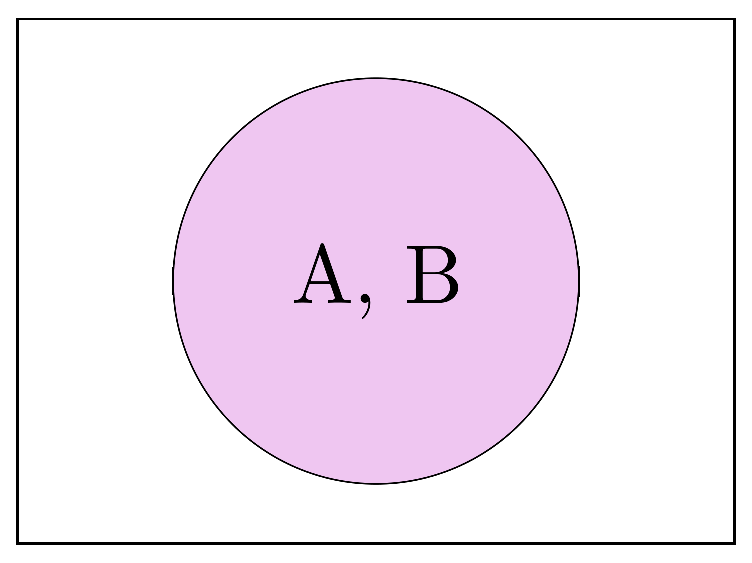
\includegraphics[width=0.2\textwidth]{discrete/sets/equal.eps}
  \end{center}
  \caption{$A=B$.}
\end{figure}
We have two ways to write an \textbf{empty set}.
We could write $\emptyset$ or $\{ \}$.

A set with only one element is called a \textbf{singleton set}.\index{singleton set}

The set $A$ is a \textbf{subset}\index{subset} of set $B$ iff
\[ \forall x (x \in A \implies x \in B) \]
We then write $A \subseteq B$ to show that $A$ is a subset of $B$.
To demonstrate that $A$ is a subset of $B$, show that if $x$ belongs to $A$ then it also belongs to $B$.
To show that $A$ is not a subset of $B$, that is, $A \not \subseteq B$, find a single element $x \in A$ such that $x \not \in B$.
\footnote{The symbol $\not \in$ means \emph{not in}.}
\begin{figure}[H]
  \begin{center}
    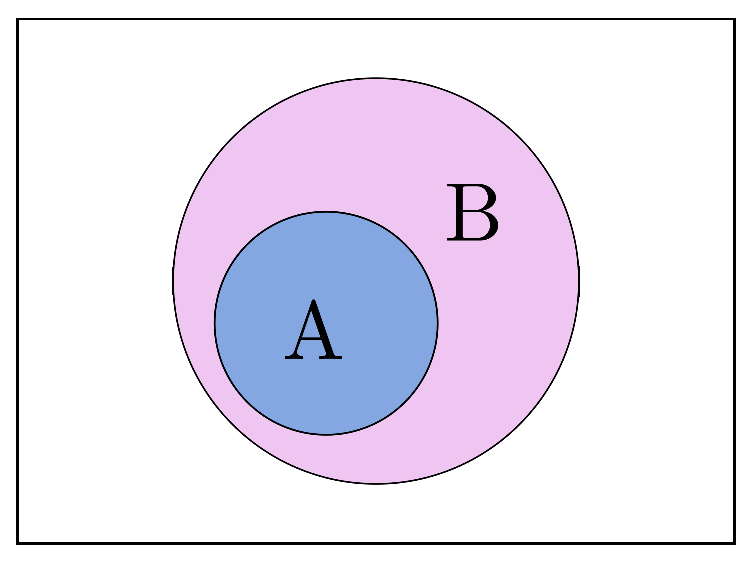
\includegraphics[width=0.2\textwidth]{discrete/sets/subset.eps}
  \end{center}
  \caption{$A\subseteq B$}
\end{figure}
If the set $A$ is a subset of the set $B$ but $A \neq B$, we write $A \subset B$ and say that $A$ is a \textbf{proper subset} of $B$.
That is, $A$ is a proper subset of $B$ iff
\[ \forall x (x \in A \implies x \in B) \land \exists x (x \in B \and x \not \in A). \]
This means, if the element $x$ exists in set $A$, then it also exists in set $B$, but there is at least one element $x$ in $B$ that is not in $A$.

\subsection{Set Operations}

For a set $A$ and a set $B$, the following operations apply:

The \textbf{cartesian product} of $A$ and $B$, denoted $A \times B$, is the set of all ordered pairs $(a, b)$ where $a \in A$ and $b \in B$. Hence,
\[ A \times B = \big\{ (a,b) | a \in A \land b \in B \big\} \]

\begin{ex}
  Find $A \times B$ when $A = \{ 1,2 \} $ and $B = \{ a, b, c\} $.
  \begin{sol}
    \[A \times B = \big\{(1,a),(1,b),(1,c),
    (2,a),(2,b),(2,c)\big\}\]
  \end{sol}
\end{ex}

The \textbf{intersection}\index{intersection} of $A$ and $B$, denoted $A \cap B$,
is the set containing those elements in both $A$ and $B$, but not just one.
If the intersection of $A$ and $B$ is $\emptyset$, we say the two sets are \textbf{disjoint}.\index{disjoint}
\[ A \cap B = \big\{ x \in A | x \in B \big\}\]
\begin{figure}[H]
  \begin{center}
    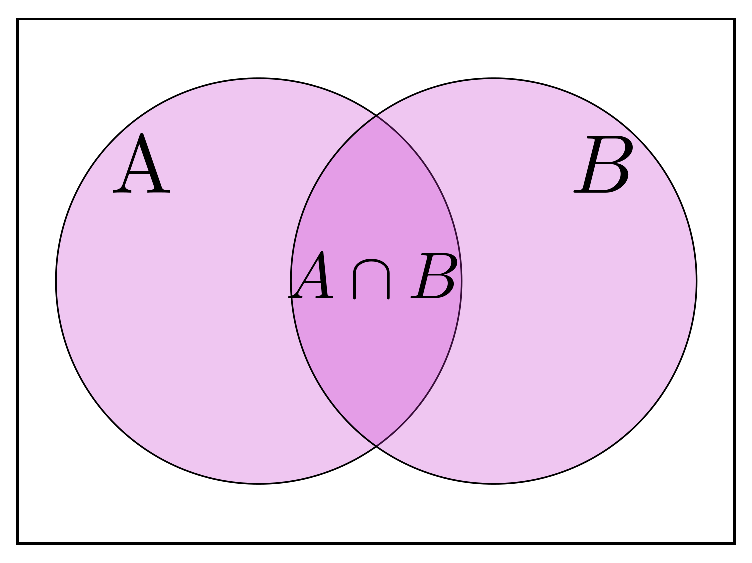
\includegraphics[width=0.2\textwidth]{discrete/sets/intersection.eps}
  \end{center}
  \caption{$A\cap B$}
\end{figure}The \textbf{union}\index{union} of $A$ and $B$, denoted $A \cup B$,
is the set containing all elements in either or both $A$ and $B$.
\[ A \cup B = \big\{ x | x \in A \lor x \in B \big\}\]
\begin{figure}[H]
  \begin{center}
    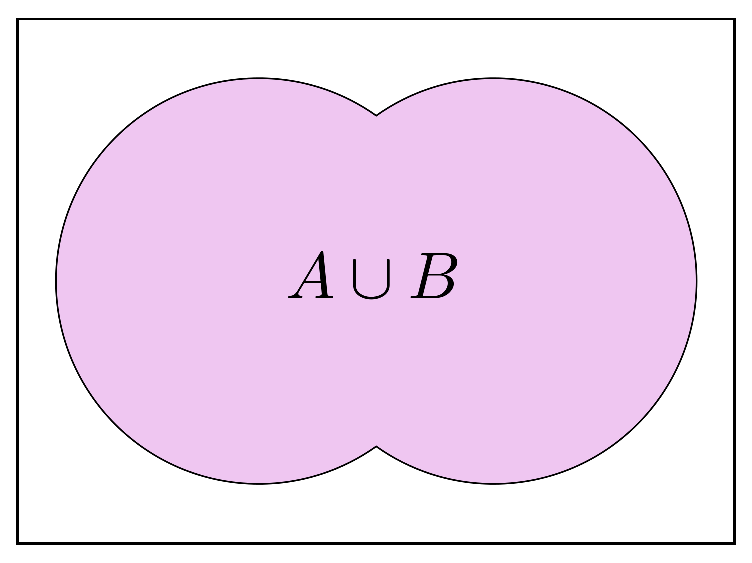
\includegraphics[width=0.2\textwidth]{discrete/sets/union.eps}
  \end{center}
  \caption{$A \cup B$}
\end{figure}
The \textbf{complement}\index{complement} of $A$ and $B$, denoted $A \setminus B$,
is the set containing those elements in $A$ but not in $B$.
It is sometimes called the \emph{component of $B$ with respect to $A$}.
This phrasing is used because the difference of $A$ and $B$ is different from the difference of $B$ and $A$.
\[ A \setminus B = \big\{ x \in A \big| x \not\in B \big\} \]

The \textbf{absolute complement}\index{absolute complement}
of $A$ is denoted $A^c$, and exists only if a universal set\footnote{A set containing all sets, including itself.}
$\mathbf{U}$ is defined, and is found by
\[ A^c = \mathbf{U} \setminus A.\]

\begin{table}
  \centering
    \begin{tabular}{>\(l<\) r}
      \textbf{Proposition} & \textbf{Name} \\ \hline\noalign{\smallskip}
      A \cap U = A & \multirow{2}{*}{identity laws} \\
      A \cup \emptyset = A \\\hline
      A \cup U = U & \multirow{2}{*}{domination laws} \\
      A \cap \emptyset = \emptyset \\\hline
      A \cup A = A & \multirow{2}{*}{idempotent laws} \\
      A \cap A = A \\\hline\noalign{\smallskip}
      \big(A^c\big)^c=A & involution law \\\noalign{\smallskip}\hline
      A \cup B = B \cup A & \multirow{2}{*}{commutative laws} \\
      A \cap B = B \cap A \\\hline
      A \cup (B \cup C) = (A \cup B) \cup C & \multirow{2}{*}{associative laws} \\
      A \cap (B \cap C) = (A \cap B) \cup C\\\hline
      A \cup (B \cap C) = (A \cup B) \cap (A \cup C) & \multirow{2}{*}{distributive laws} \\
      A \cap (B \cup C) = (A \cap B) \cup (A \cap C) \\\hline\noalign{\smallskip}
      \big(A \cup B\big)^c = A^c \cap B^c & \multirow{2}{*}{DeMorgan's laws} \\
      \big(A \cap B\big)^c = A^c \cup B^c \\\hline
      A \cup (A \cap B) = A & \multirow{2}{*}{absorbtion laws} \\
      A \cap (A \cup B) = A \\\hline
      A \cup A^c = U& \multirow{2}{*}{complement laws} \\
      A \cap A^c = \emptyset
    \end{tabular}
  \caption{Useful set identities.}
  \label{tab:setidentities}
\end{table}


\section{The Well-Ordering Principle}\index{well-ordering principle}
The \textbf{well-ordering principle} states that
\begin{theorem}
Every nonempty set of nonnegative integers has a smallest element.
\label{thm:wellordered}
\end{theorem}
We can use this to prove propositional statements associated with universal quantifiers.

To prove that
\[ \forall n \in \mathbb N \big( P(n)\big) \]
First, we define a set $C$ such that
\[ C : : = \big\{ n \in \mathbb N^+ \big| \neg P(n) \big\} \]
That is, we define the set $C$ to be the set of integers for which $P(n)$ is false.
We assume that this set is nonempty---that is, there is at least one nonnegative integer for which $P(n)$ is false.
By the well-ordering principle, there is a smallest element, $n$, in $C$.
From this, we reach a contradiction.
For example, we could show that $n$ can be used to find an element smaller than itself.
Now, we conclude that the set $C$ must be empty.

\begin{ex}
  Prove that the sum of all integers from $1$ to $n$ is \[\frac{n(n+1)}{2}.\]

  In basic algebraic notation, we could write this sum as
  \[1 + 2 + 3 + \cdots + n \]
  But we have a way of simplifying this using something called \textbf{sigma notation}\index{sigma notation}.
  We would write it as follows:
  \[1+2+3+\cdots+n  \sum_{1}^n \frac{n(n+1)}{2} \]
  \begin{proof}
    Now, we define a set $C$ such that
    \[ C : : = \bigg\{ n \in \mathbb N \big| \sum_{i=1}^n i \neq \frac{n(n+1)}{2}\bigg\}\]
    By the \emph{well-ordering principle}, $C$ has a smallest element, which we will call $c$.
    Since $c$ is the smallest counterexample,
    \[\sum_{i=1}^n = \frac{n(n+1)}{2}\]
    holds for all $n<c$ but not for $n=c$. So, that sum should hold for $c-1$:
    \begin{align*}
      1+2+3+\cdots+(c-1)&=\frac{(c-1)\big[(c-1)+1\big]}{2}\\
      1+2+3+\cdots+(c-1)&=\frac{(c-1)c}{2}\\
      1+2+3+\cdots+(c-1)&=\frac{c^2-c}{2}\\
      \intertext{Now, we add $c$ to both sides.}
      1+2+3+\cdots+(c-1)+c&=\frac{c^2-c}{2}+c\\
      \intertext{Simplify.}
      1+2+3+\cdots+(c-1)+c&=\frac{c^2-c}{2}+(c)\left(\frac{2}{2}\right)\\
      1+2+3+\cdots+(c-1)+c&=\frac{c^2-c+2c}{2} \\
      1+2+3+\cdots+(c-1)+c&=\frac{c^2+c}{2} \\
      \intertext{Factor out $c$ from the right-hand side.}
      1+2+3+\cdots+(c-1)+c&=\frac{c(c+1)}{2} \\
    \end{align*}
    Which means that
    \[\sum_{i=1}^n = \frac{n(n+1)}{2}\]
    holds for $c$, which contradicts our definition of $C$. Therefore $P(n)$ holds for all  $n \in \mathbb N$.
  \end{proof}
\cite{mcsfull}
\end{ex}

A few theorems come from the \emph{well-ordered principle}:\footnote{Proofs will come. From \cite[29]{mcsfull}.}
\begin{theorem}
  Any set of integers with a lower bound is well-ordered.
\end{theorem}
\begin{theorem}
  Any nonempty set of integers with an upper bound has a maximum integer.
\end{theorem}
